\documentclass{article}
\usepackage{graphicx} % Required for inserting images
\usepackage{amsmath}
\usepackage[english, russian] {babel}
\usepackage[utf8]{inputenc}
\usepackage[T2A]{fontenc}
\usepackage{minted}
\usepackage{float}
\usepackage{amssymb}

\title{Методы вычислений}
\author{silvia.lesnaia }


\begin{document}

\maketitle

\textbf{02.09.25}

\section{1 Раздел}
\textbf{Интерполяция функций одного аргумента}

Интерполяция - приближение.

\subsection{Параграф 1 - Постановка интерполяций}

Пусть заданна дискретным набором своих значений некоторая функция f 
а именно, данная функция определенна следующией таблицей своих значений 

тут пикча с табличкой 


, где $f_k=f(xk),\bigvee k =\overline{0,n} $

требуется указать(построить ) непрерывную на некоторой области функцию g(x)
такую что бы выполнялись следующие условия:  

\textbf{$g(x_k)=f_k,\bigvee k =\overline{0,n}$ (1) (ГУИ)}

\begin{figure} [H]
    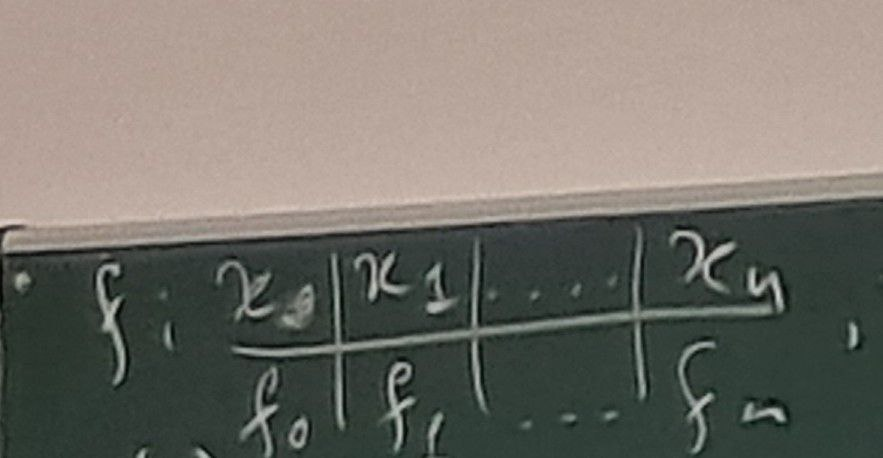
\includegraphics[width=0.50\linewidth]{photo_5310113942493852121_y.jpg}
\end{figure}

\begin{figure} [H]
    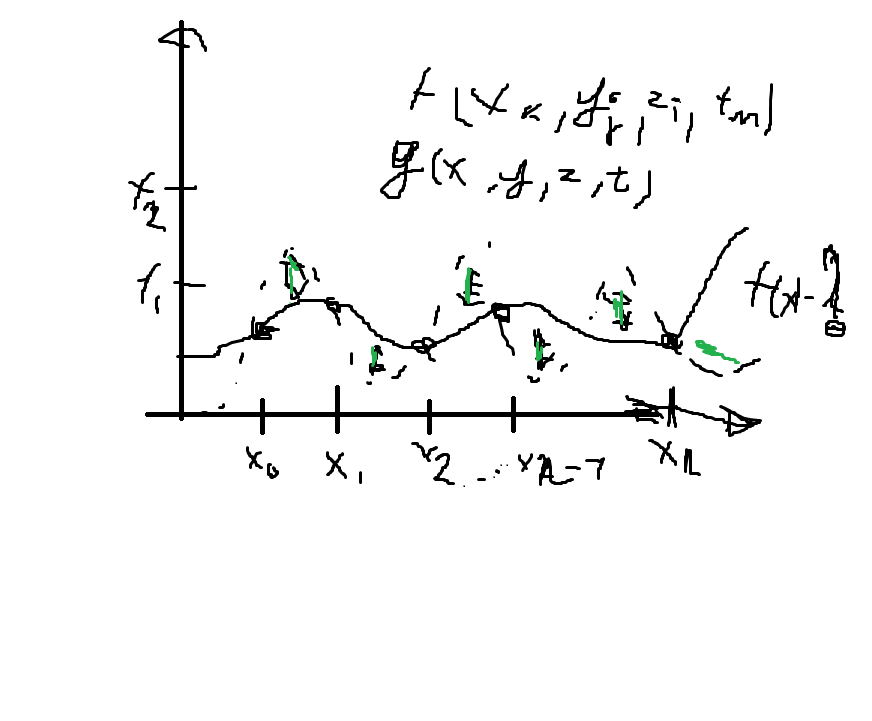
\includegraphics[width=0.80\linewidth]{Без имени.png}
\end{figure}


01 x,x1,...x2 б.н будем называть \textbf{узлами интерполяций(узлами приближений)}

\vspace{3mm}

02 f (xk,fk), $\bigvee k =\overline{0,n}$ называется \textbf{интерпоплируемой(приближаемой) функций}

\vspace{3mm}

03 g(x) удовлетворяющей условиям (1) будем называть \textbf{интерполирующией
(приблежающий, интерполяционный) или  интерполянта }

\vspace{3mm}

04 условия (1) будем называть \textbf{главным условием интерполяции(ГУИ)}

\vspace{3mm}


В сформулированной задачи интерполции очевидно в качестве искомой интерполянты
\underline{ бесконечной количество искомой функции} 

\begin{figure} [H]
    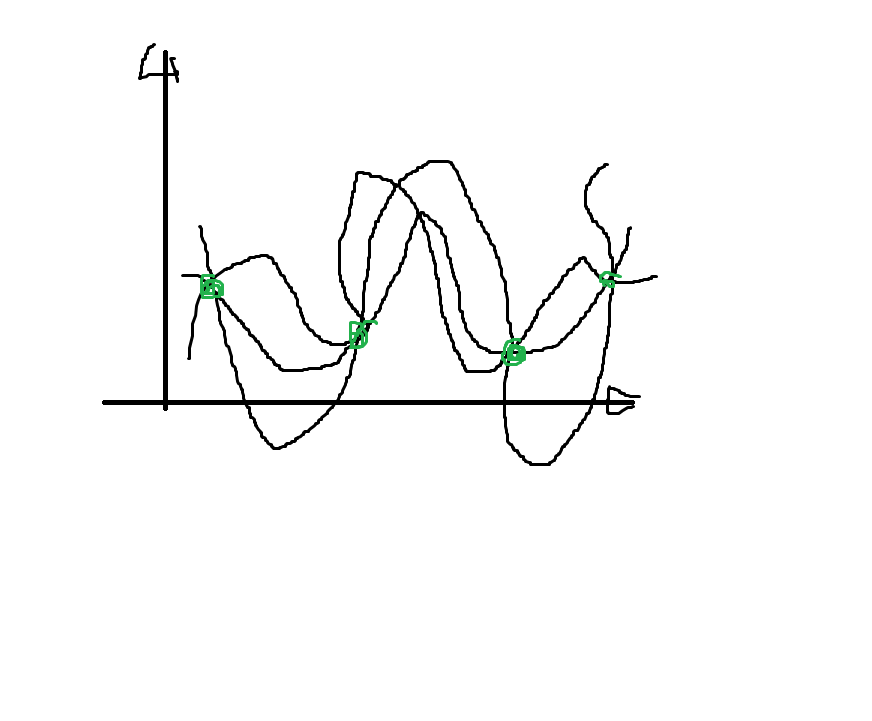
\includegraphics[width=0.50\linewidth]{Без имени1.png}
\end{figure}


\subsection{Параграф - 2  Интерполяционный многочлен в общем виде}

В этом параграфе покажем что в качестве искомой интерполяный - задачи интерполяции(З.И)
может быть предложен алгебраический многочлен в степени n,
построенный по (n+1)-му по парно различному узлу интерполяции.

\vspace{3mm}



Такми образом для (n+1) узла интерполции  $x_0,x_1,...x_n$  осторожно попробуем построить
алгебраический многочлен $\rho_n(x) = a_nx+a_{n-1} -1 ... + a_1x^1+a_0$ (2)

Потребуем что бы алгебраический многочлен вида (2) удовлетворял ГУИ (1)

а именно что бы 

$\rho_n(x_0)=f_0$        \hspace{2mm} (2)          \hspace{5mm}   $a_x0^n+a_{n-1}x^{n-1}_0+...+a_1x_0+a_0=f_0$  

$\rho_n(x_1)=f_1$       \hspace{2mm}    $\Leftrightarrow $ \hspace{5mm}   $a_nx_1^n+a_{n-1}x^{n-1}_1+...+a_1x_1+a_1=f_1$  (3)

и т.д 

$\rho_n(x_n)=f_n$ \hspace{10mm} $a_n x_n^n+a_{n-1}x^{n-1}_n +...+a_1x_n+a_0=f_n$



Равенство (3) по своей алгебраической природе предствалвеют собой СЛАУ
(система линейных алгебраических уравнений) раззмеронсти 

СЛАУ$(n+1)x(n+1)$ отн. несущ.коэф.


Что бы решить СЛАУ (3) 

запишем определить $\Delta_3 =$
$\begin{pmatrix}$
$x_0^n & x_0^{n-1} & \cdots & x_0 & 1 \\$
$x_1^n & x_1^{n-1} & \cdots & x_1 & 1 \\$
$\vdots & \vdots & \ddots & \vdots & \vdots \\$
$x_n^n & x_n^{n-1} & \cdots & x_n & 1$
$\end{pmatrix}$

$=\dots \prod (x_j-x_i)\neq 0 $ (4)


Что бы определитель (4) нужно чтоб узел $x_j\neq x_i, если j\neq i$ (5)
это есть условие по парной различности узлов интерполции


Таким образом из выше изложенного можем получить следующие:

Определитель (4) отличен от нуля при условии (5), а седовательно СЛАУ (3) решив 
каким либо подходящим численным методом, сможем найти ее единтсвенное решение,
а именно значение искомых коэффицентов $a_0,a_1$

Найдя эти коэффиценты  и подставим их в искомое (2) явно аналитическую формулу для искоомого
предтсваления интерполянты:

$\rho_n(x_n)=a_nx^n+a_{n_1}+x^{n-1} + a_1x+a_0$




Тут должна быть лекция, но я не смогла

\textbf{23.09.25}


графики стерли я не успела

гг



\vspace{10mm}

\begin{figure} [H]
    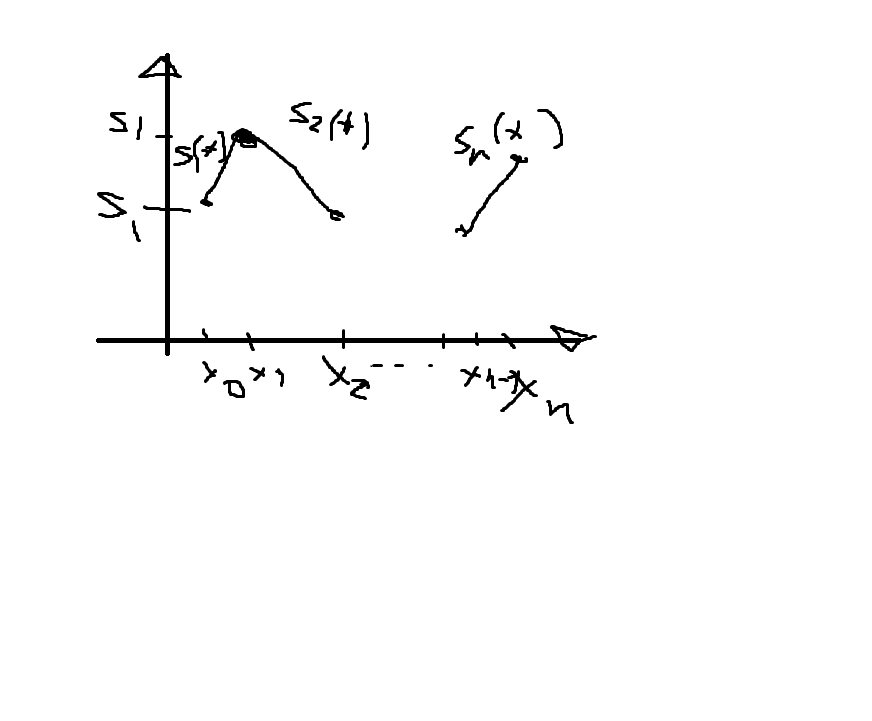
\includegraphics[width=0.70\linewidth]{Без име2ни.png}
\end{figure}


$S_i (x)=a_i+b_i(x-x_{i-1})+c_i(x-x_{i-1})^2+d_i(x-x_{i-1})^3 $ (1)

$x \in (x_{i-1}, x_i)$


На каждом отрезке сформирован соседними узлами интерпоялции, определим
некоторой алгебраический многочлен третьей степени вида (1).

И поскольку каждый такой многочлен будем рассматривать исключительно на соответствущем
отрезке будем называть \textbf{кубическим сплаином} или алгебраическим многочленом третьей степени.

Сплайн - кусок, фрагмент чего либо.


\begin{figure} [H]
    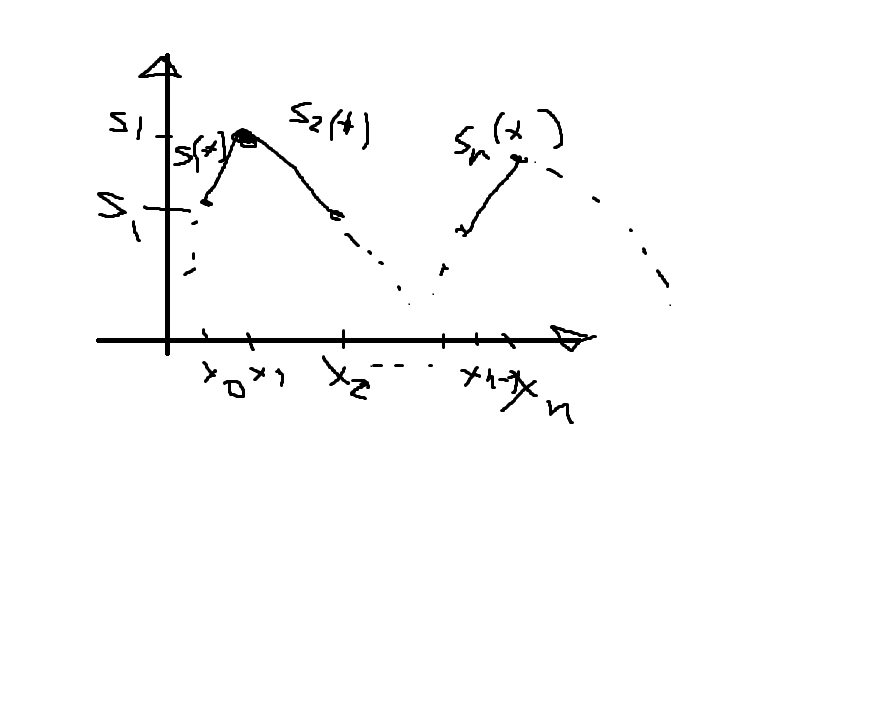
\includegraphics[width=0.70\linewidth]{Без име24ни.png}
\end{figure}

\begin{figure} [H]
    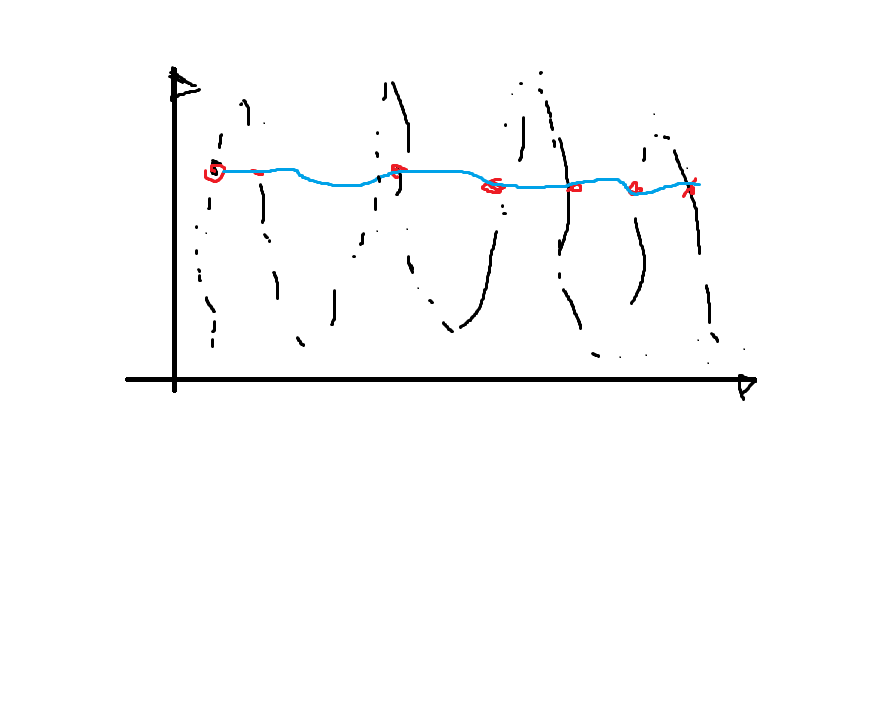
\includegraphics[width=0.70\linewidth]{Без имени7.png}
\end{figure}


Потребуем что бы кусочная "склейка", указана кубических многочленов удовлетворила главному
условию интерполяции. А именно что бы каждый сплайн вида (1) удовлетворял следующем
равенствам.

Каждый левый сплайн должен пппринимать занчения левой точки(1)\dots

$$
\begin{cases}
    S_i (x_{i-1}) = f_{i-1}, & \quad i = \overline{1, n}  \\
    S_i (x_i) = f_i, & \quad i = \overline{1, n}
\end{cases}
\Leftrightarrow
\begin{cases}
    a_i = f_{i-1}, & \quad i = \overline{1, n}  \\
    a_i + b_i * h + c_i * h^2 + \alpha * h^3 = f_i, & \quad i = \overline{1, n}
\end{cases}
$$

CЛАУ относительно нев.выраж ${a_i,b_i,c_i,d_i}_{i= \overline{i,n}}$ (2) ур, отн 4n непр


Недостающие уравнения будем строить требуя не только не прирывной склейки самих  сплаинов, 
но и не прерывной склейки их производных в тех точках.

Для удобсвто дальнейшего использования заполним следующию таблицу
\begin{figure} [H]
    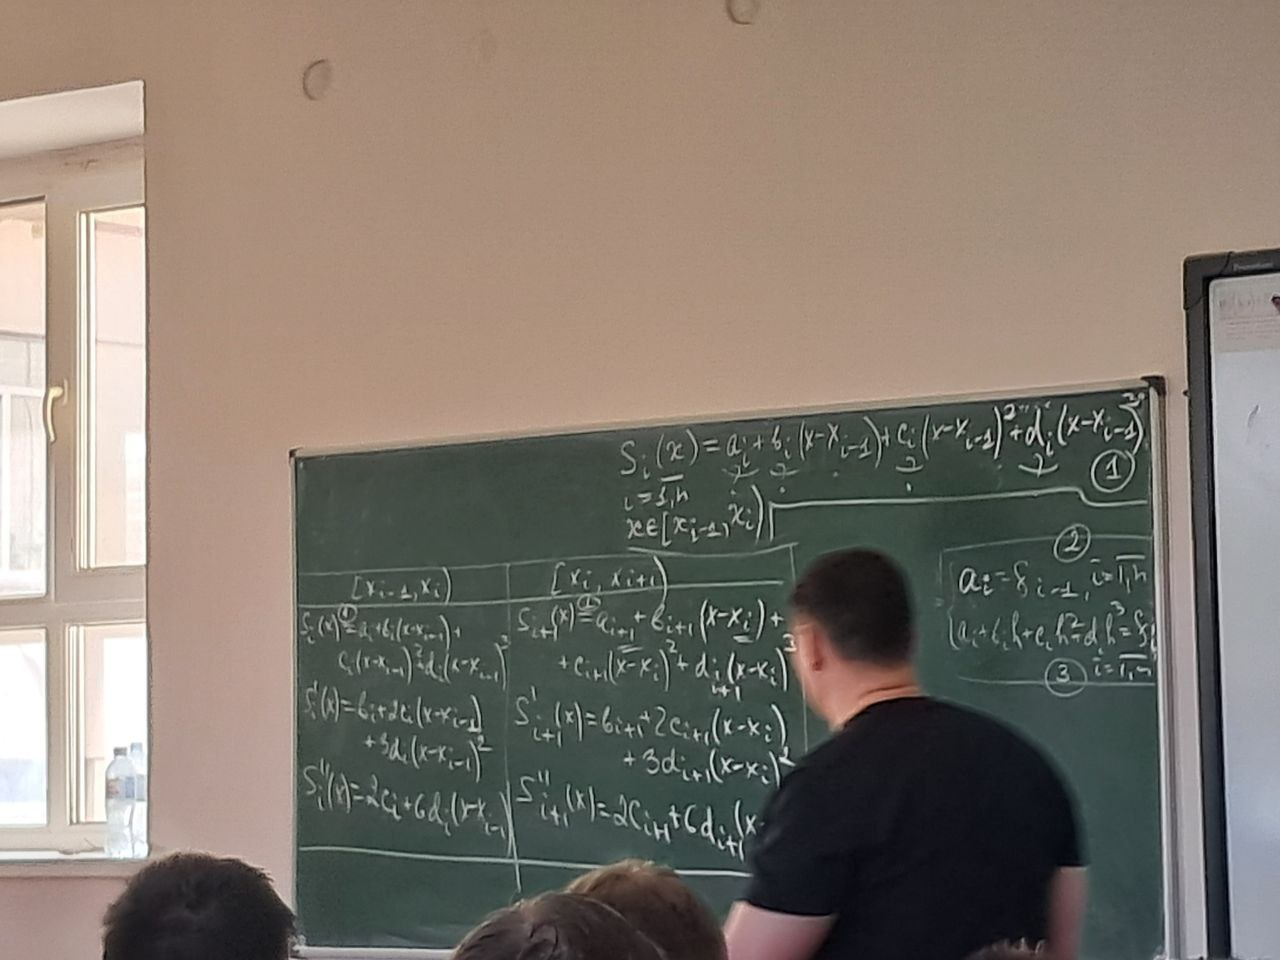
\includegraphics[width=0.70\linewidth]{photo_5375068150250467856_y.jpg}
\end{figure}


\begin{figure} [H]
    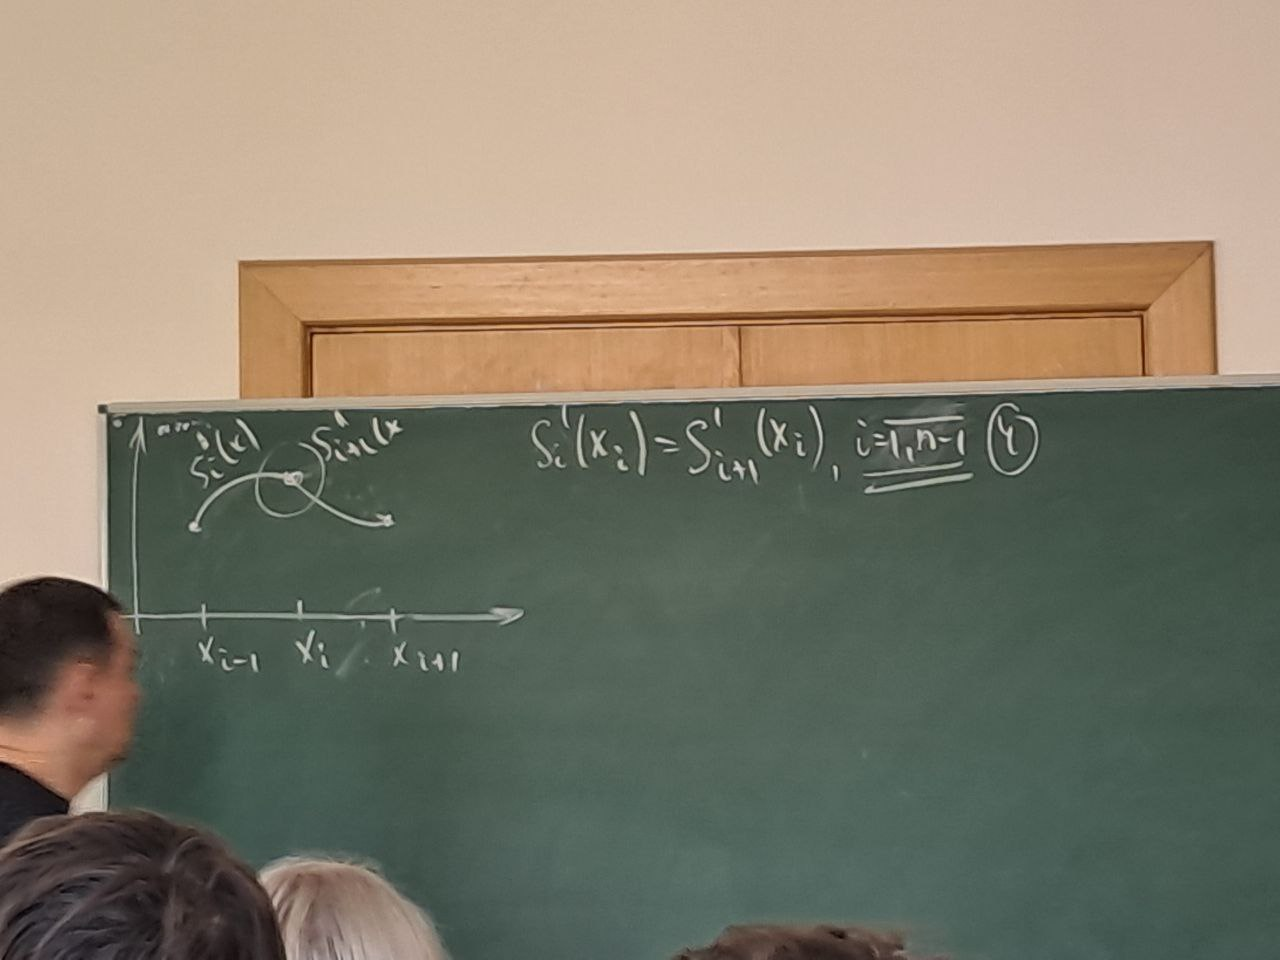
\includegraphics[width=0.70\linewidth]{photo_5375068150250467857_y.jpg}
\end{figure}


\vspace{20mm}

\textbf{07.10.25}

$a_{11} \neq 0, a_{22}^{(1)} \neq 0, a_{33}^{(2)} \neq 0,... a_{nn}^{(n-1)} \neq 0$

Соответсвенно если на каждом прямого хода мы встретим элемент $a_{kk_1}^{(k-1)} \equiv 0$ 
$(a_{kk_1}^{(k-1)} \in 0_\delta = (-\delta; \delta))$

Любое число из этого интеравала будет 0

\begin{figure} [H]
    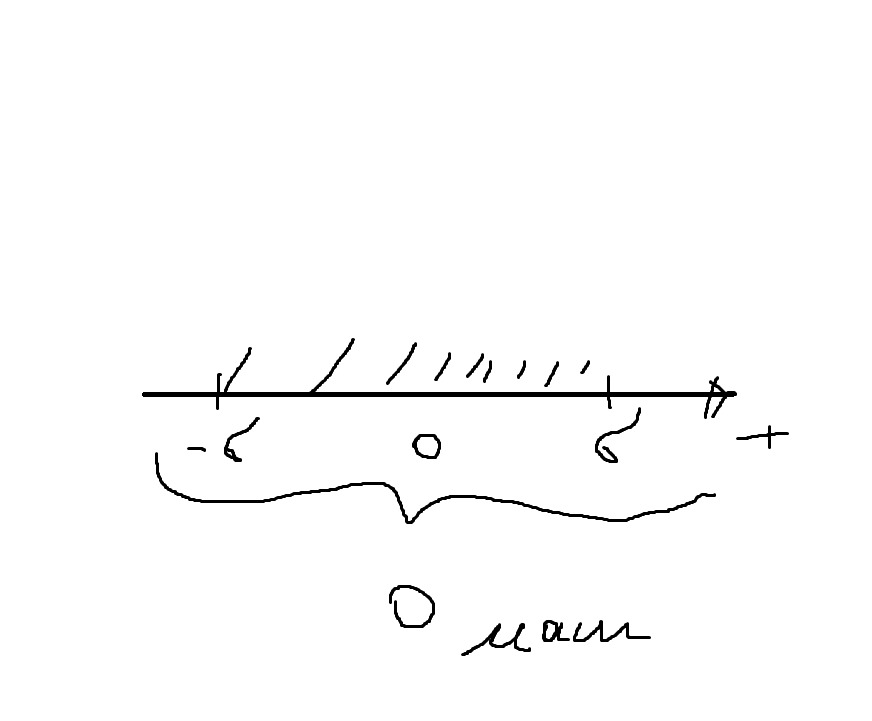
\includegraphics[width=0.70\linewidth]{Без имени8.png}
\end{figure}

\end{document}